\subsection{写真撮影画面}
写真撮影画面ではiPhoneに内蔵されているカメラを使用して観光スポットの写真を撮影する。本画面の意図は、カードリスト画面で木古内町の魅力を知り、観光スポットを訪れたユーザにそこを訪れた記念を残してもらうことである。本画面へは、カードリスト画面のカメラボタンをタップすることで遷移する。遷移してきた直後の画面を図6.3(a)で示す。写真の撮影は、画面の下の中央にある丸いボタンをタップして行う。撮影時は左上のボタンによりフラッシュの有無を選択できる。右上のボタンでは、インカメラとアウトカメラの切り替えをすることができる。また、左下の「キャンセル」ボタンをタップすることで本画面からカードリスト画面へ戻ることができる。\\ 
撮影後は、撮影した写真を保存するか再撮影を行うかを選択する画面へ遷移する。撮影後の画面を図6.3(b)で示す。右下の「写真を使用」ボタンをタップすることで写真の保存が行える。保存した場合は、撮った場所に対応するカードに上書きされ、表示される。また、写真を撮り直す場合は、左下の「再撮影」ボタンをタップすることで撮影時の画面に戻ることができる。
\newpage

\begin{figure}[htbp]
  \begin{center}
    \begin{tabular}{c}

      % 1
      \begin{minipage}{0.33\hsize}
        \begin{center}
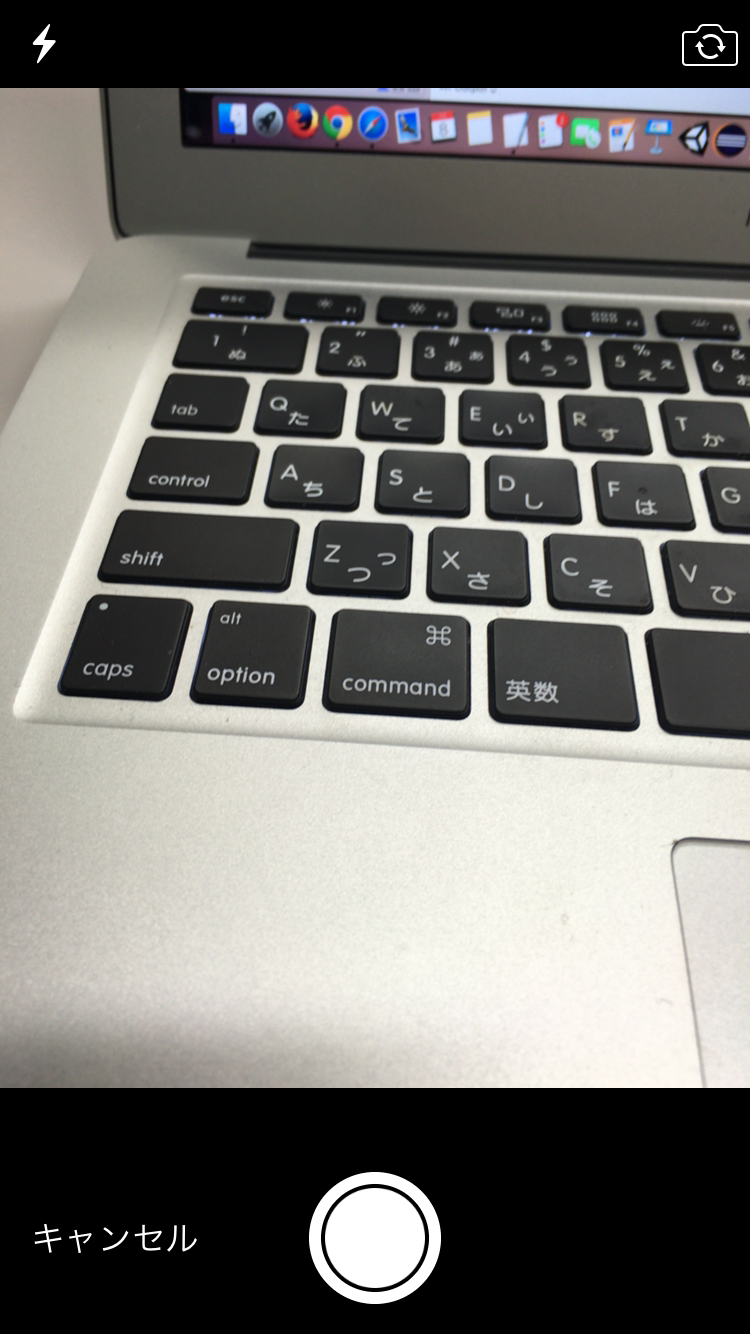
\includegraphics[width=4cm, bb=0 0 304 570]{kiko_takephoto1.PNG}
          \hspace{1cm} %(a)撮影時
          {\footnotesize (a)撮影時}
        \end{center}
      \end{minipage}

      % 2
      \begin{minipage}{0.33\hsize}
        \begin{center}
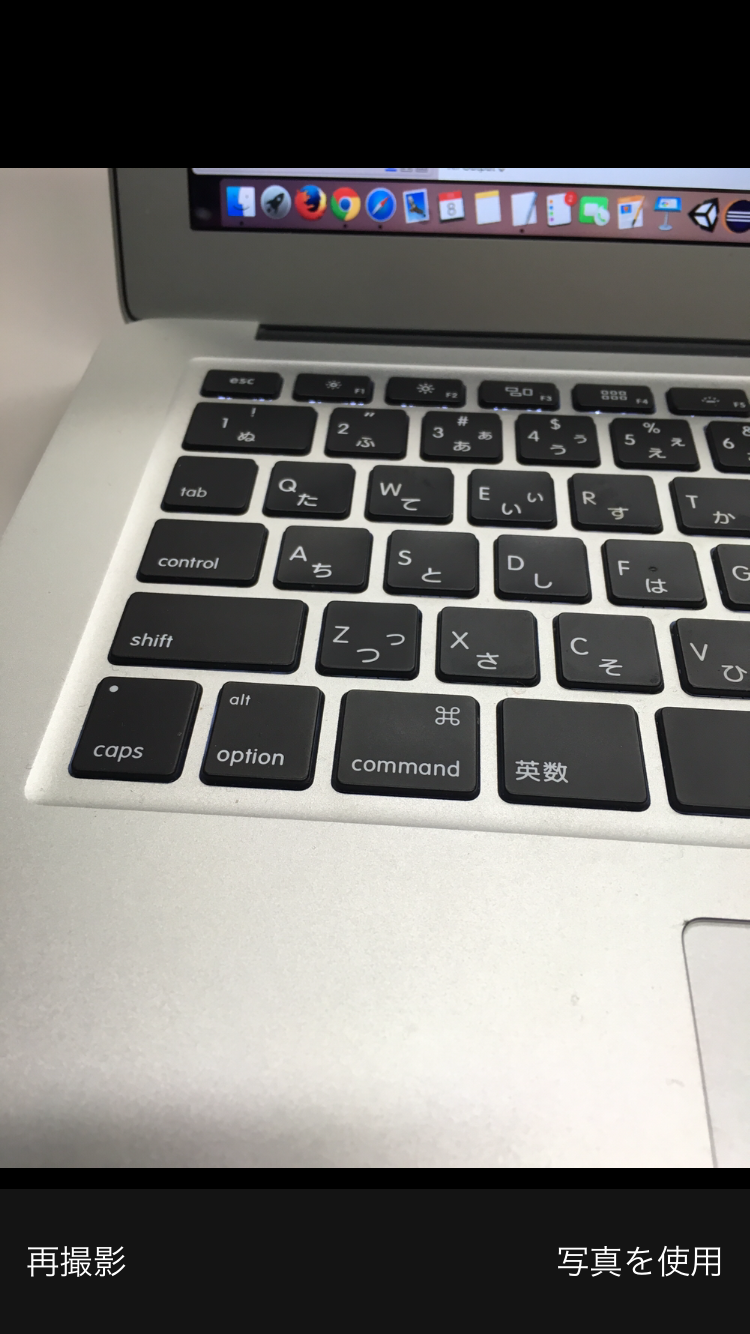
\includegraphics[width=4cm, bb=0 0 304 570]{kiko_takephoto2.PNG}
          \hspace{1cm} %(b)撮影後
          {\footnotesize (b)撮影後}
        \end{center}
      \end{minipage}
      
    \end{tabular}
    \caption{写真を撮影する機能の画面}
    \label{fig:lena}
  \end{center}
\end{figure}          

\bunseki{池田俊輝}